\documentclass[11pt,letterpaper,final]{report}
\usepackage[utf8]{inputenc}
\usepackage[francais]{babel}
\usepackage[T1]{fontenc}
\usepackage{amsmath}
\usepackage{amsfonts}
\usepackage{amssymb}
\usepackage{graphicx}
\usepackage{lmodern}
\usepackage[left=2.54cm,right=2.54cm,top=2.54cm,bottom=2.54cm]{geometry}
\begin{document}
\chapter{Cross validation entre les différentes plateformes de simulations}
\section{Validation Psim/SPS}
\subsection{Calcul de la tension moyenne}

Commençons par discuter des différences obtenues entre les différentes simulations. On a remarqué que la fonction "Mean" dans simulink et Psim ne donne pas le même résulat. Pour le montrer, on a testé chacune des deux fonctions avec un sinus 100Vamplitude, 50Vmoy et à 1KHz de fréquence. Les figures~\ref{dis_mean} et \ref{D_mean} montre les résulats obtenus avec une fréquence de 500Hz du moyenneur.



\begin{figure}[h]
\centering
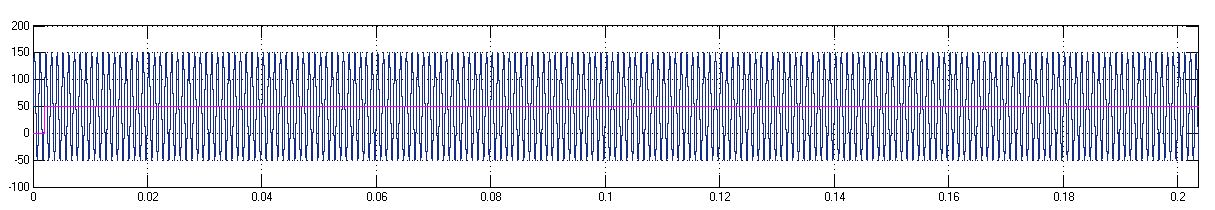
\includegraphics[scale=0.5]{fig/moy_sim.jpg}
\caption{Réponse de la function "Discrete Mean" sur SPS}
\label{dis_mean}
\end{figure}

\begin{figure}[h]
\centering
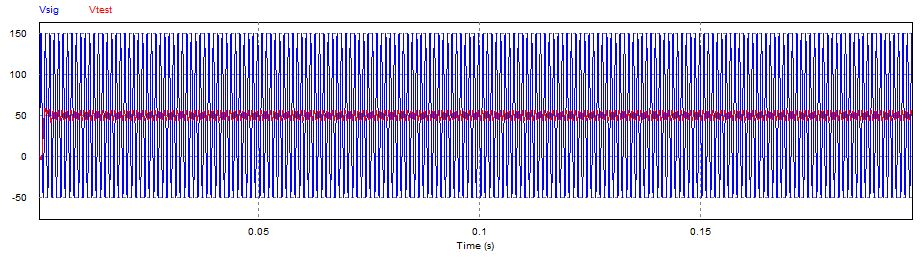
\includegraphics[scale=0.5]{fig/moy_psim.jpg}
\caption{Réponse du bloc "DC Voltmeter" sur PSIM}
\label{D_mean}
\end{figure}


\begin{figure}[ht]
\centering
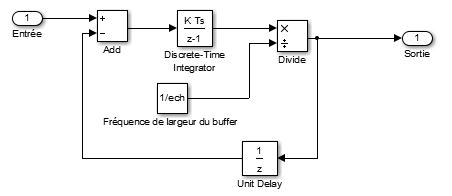
\includegraphics[scale=0.8]{fig/moy.jpg}
\caption{Fonction de moyennage de la tension}
\label{moy}
\end{figure}
On remarque bien que les résultats sont différents dans les figures~\ref{dis_mean} et \ref{D_mean}. La tension moyenne calculé sur simulink est plus précise  et varie moins que celle de Psim. La précision est telle que le résultat de Psim est variant sur chaque période tandis que celle de simulink a une apparence droite. Par contre, le temps de réponse de simulink est plus long que celui de Psim qui répond très rapidement. Par conséquent, on a décidé de monter notre propre fonction de moyennage pour avoir un fonctionnement pareille dans les deux simulations. La figure~\ref{moy} représente la fonction qui est constitué d'un intégrateur à gain équivalent au pas de calcul qui est de
\begin{equation}
Ts = 10^{-5}
\end{equation} avec un retour et un gain qui contrôle la sensibilité de la fonction, on a mis 1/3000 pour avoir le meilleur résultat. De plus, on cascadé 10 fonctions intégrateur pour optimiser le résultat et avoir une moyenne plus ou moins en continu.





\begin{figure}[ht]
\centering
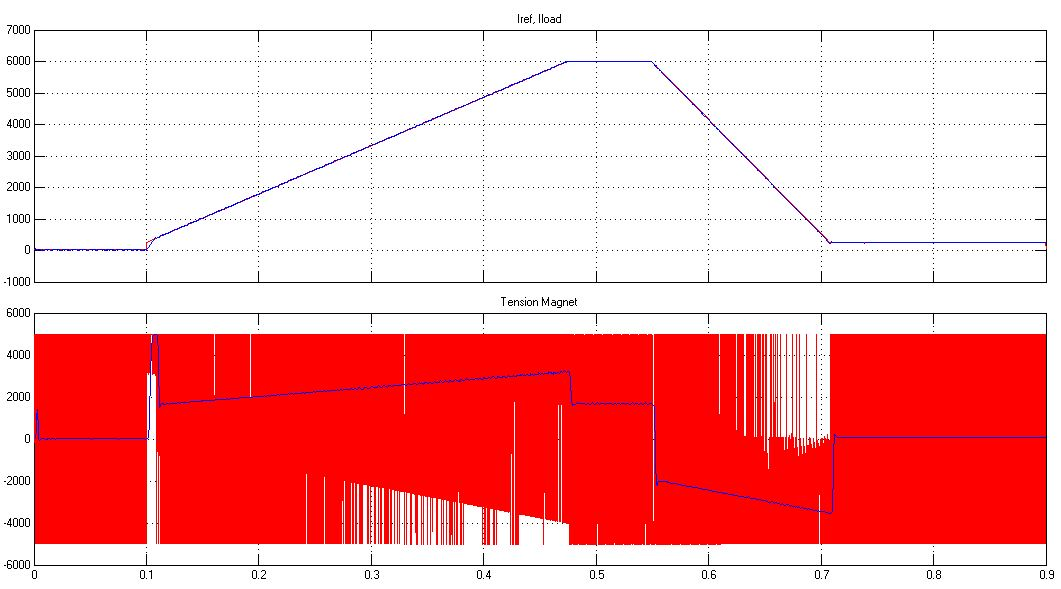
\includegraphics[scale=0.5]{fig/resul_sim.jpg}
\caption{Résultats de simulation sur SIMULINK}
\end{figure}
\begin{figure}[ht]
\centering
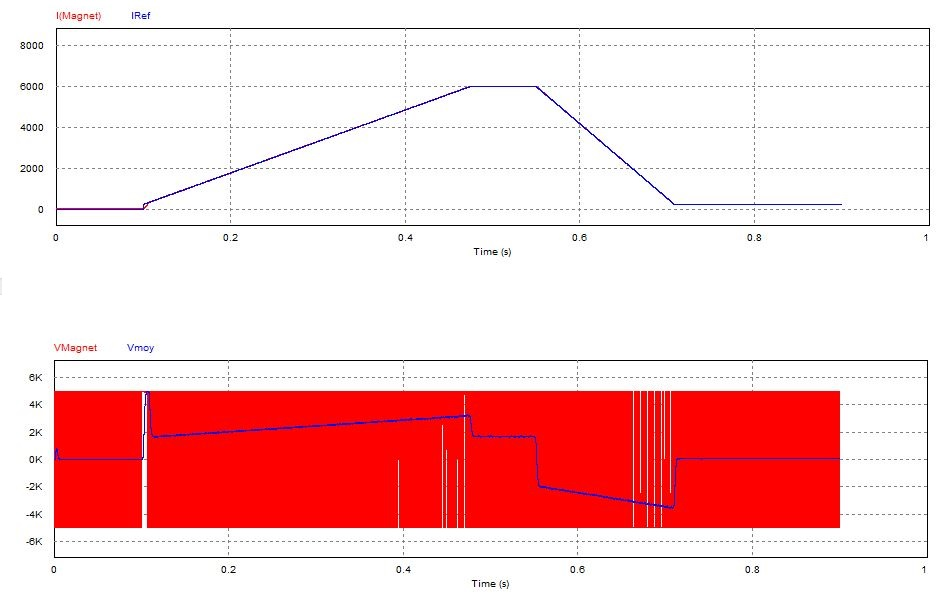
\includegraphics[scale=0.6]{fig/resul_psim.jpg}
\caption{Résultats de simulation sur Psim}
\end{figure}

\begin{figure}[ht]
\centering
\includegraphics[scale=0.5]{erreur_PSIM.jpg}
\caption{La différence entre la référence de courant et la valeur obtenu pour PSIM}
\end{figure}

\begin{figure}[ht]
\centering
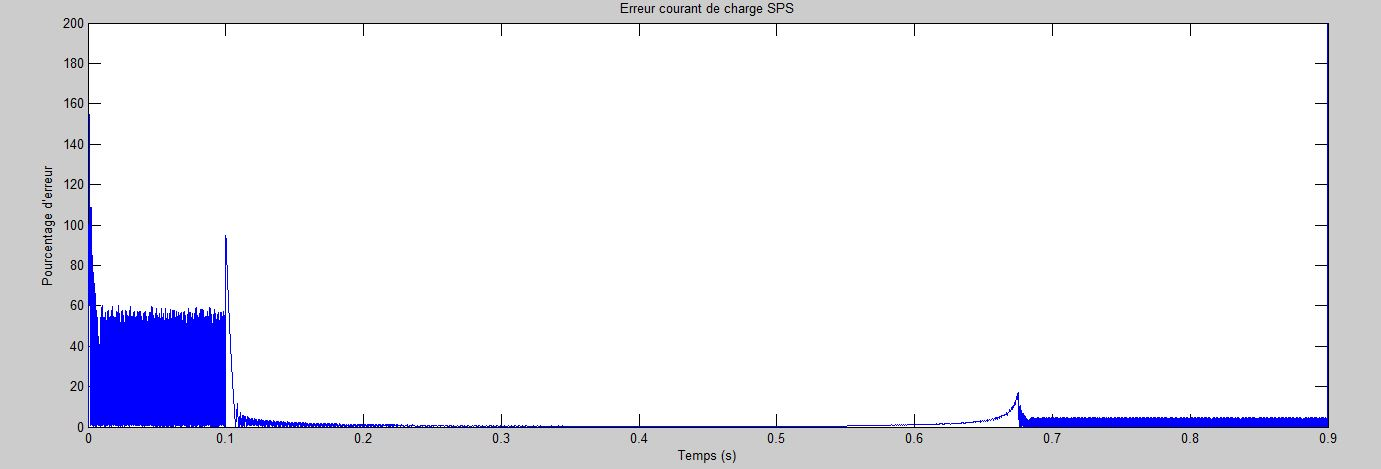
\includegraphics[scale=0.5]{erreur_SPS.jpg}
\caption{La différence entre la référence de courant et la valeur obtenu pour SPS}
\end{figure}

\begin{figure}[ht]
\centering
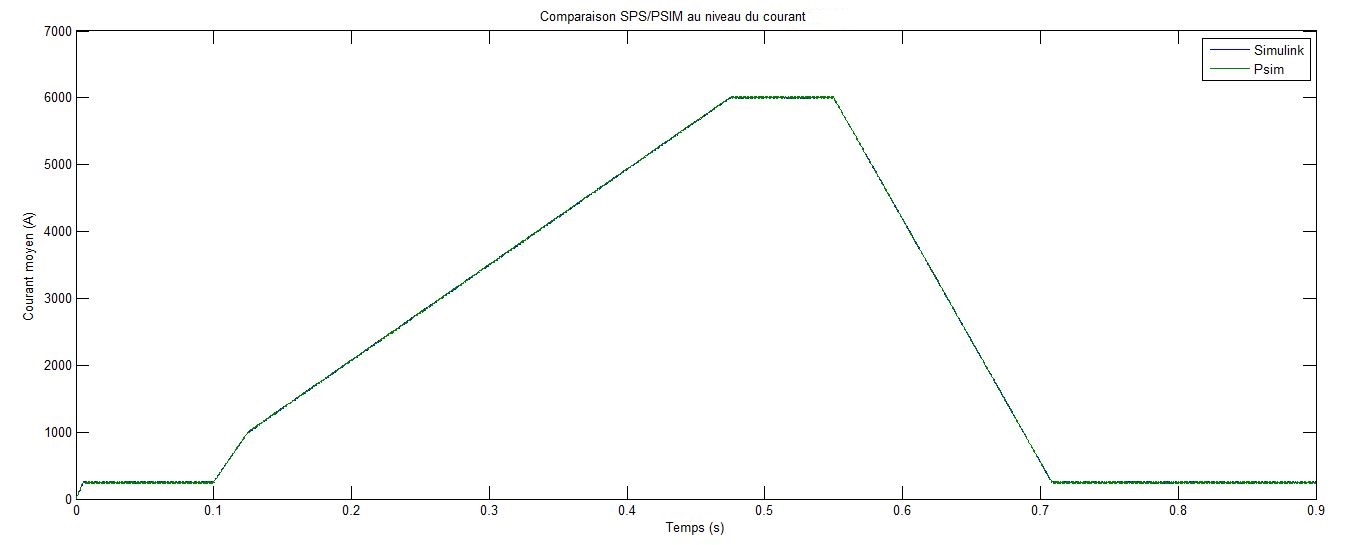
\includegraphics[scale=0.5]{comp_PSIM_SPS.jpg}
\caption{L'erreur entre PSIM et SPS}
\label{comp_PSIM_SPS}
\end{figure}
\subsection{Calcul du courant}
Nous avons comparés les deux plateformes concernant la différence par rapport au résultat du courant. Nous avons obtenu une différence de 0.011\%
entre Psim et Simulink en utilisant la valeur moyenne de courant pour le calcul en suivant l'équation~\ref{eq2}. 
\begin{equation}
Erreur = \frac{mean(I_{simulink})-mean(I_{Psim})}{mean(I_{simulink})}
\label{eq2}
\end{equation}

\end{document}